% sim_attach.tex -- Results: attach in simulation (draft 4 Oct 2026). No run ids in the text.
% Runs: network attach demo R0196/R0197, R0203/R0204, R0209 (storyboard), R0234, R0243 (10 Sep,
% 0.6 kg ring); layouts R0234, R0266-R0272; weld ladder R0126-R0141 (9 Aug); OCP attach SIL
% R0518-R0521, Gazebo R0541-R0552, R0575/R0577, R0580/R0581 (25 Sep); M1 R0646 (baseline),
% R0685/R0686, Wesley watched R0687 (27 Sep); combined M1 R0696/R0697, R0699 canonical;
% M2 T0015-T0029, bench R0707-R0720. Legacy worlds: 0.86 kg ring,
% 0.5 m rods, 0.64 kg UAVs, linear thrust map, tracker box 0.025 (all before 4 Oct).
% FIGURE TODO: rebuild the storyboard on the M1 rejoin (R0685) with tools/attach_storyboard.py.

\subsection{Attach}
\label{sec:sim_attach}

The attach was developed in three stages: a network-based attach, the attach by OCP resize, and the
full rejoin mission with the collaborator's approach controller. None has yet been flown on the rig
twin or the rig.

\subsubsection{Network attach}

\redo{the network attach during a circle at 0.2\,m/s: three UAVs at 3, 12 and 9 o'clock, ATTACH holds the target, a fourth UAV welds at 6 o'clock and is handed out by the dissipative network. With it the storyboard figure (the fleet at four instants, the plan view of the approach, the ring tilt against time).}
% --- original text, flown before the rig twin; kept to refill this place:
% The first attach demonstration (Figure~\ref{fig:attach}) used a 0.6\,kg ring. Three UAVs at 3, 12 and
% 9 o'clock flew a circle at 0.2\,m/s; ATTACH held the target, and a fourth UAV welded at 6 o'clock and
% was handed out by the dissipative network.
%
% \begin{figure}[h]
% \centering
% 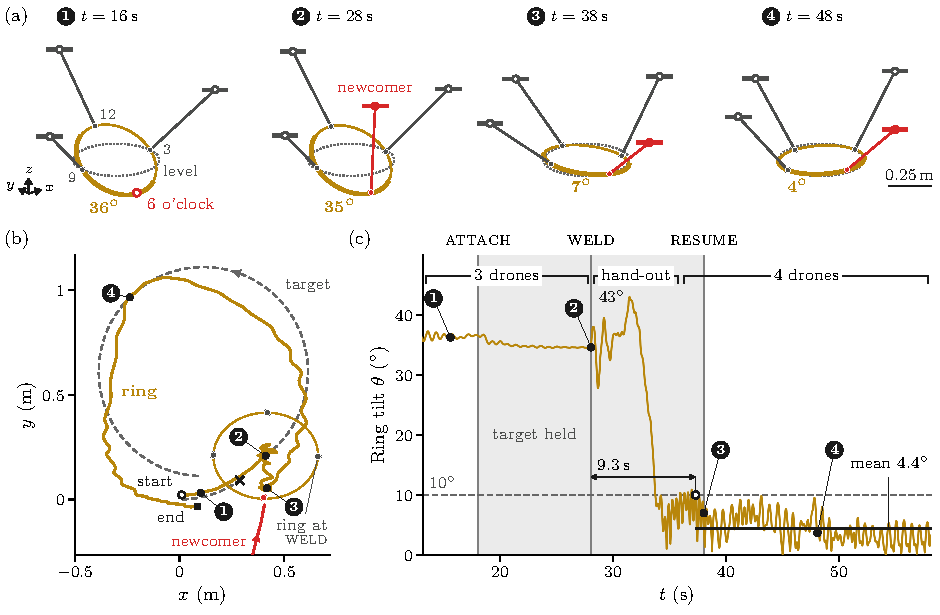
\includegraphics[width=\textwidth]{Images/attach_storyboard.pdf}
% \caption[Attach during a circle]{Attach during a circle in Gazebo (0.6\,kg ring of radius 0.25\,m on 0.5\,m rods). (a) The
% fleet at the four numbered instants, rebuilt from the logged poses in one orthographic view: carriers
% grey, newcomer red; thick: near half of the ring; dotted: the ring if it were level; bar: 0.25\,m.
% (b) Plan view of the ring centre (gold; circle: start, square: end), the payload target (dashed; x:
% held from ATTACH) and the newcomer's approach (red), with the ring and its rim anchors at the weld.
% (c) Ring tilt; grey band: target held; dashed: 10$^\circ$. Three UAVs at 3, 12 and 9 o'clock start
% the circle with the ring tilted by 34--37$^\circ$. ATTACH holds the target and the newcomer welds to
% the empty 6 o'clock rim. During the 8\,s hand-out the tilt first rises to 43$^\circ$; from 9.3\,s
% after the weld it stays under 10$^\circ$ (mean 4.4$^\circ$, peak 9.96$^\circ$), and the four UAVs fly
% the rest of the circle, 0.20\,m RMS from the target against 0.02\,m with three.}
% \label{fig:attach}
% \end{figure}

\redo{the network attach by layout, 3/12/9 o'clock against 4/12/8 o'clock with the newcomer at 6: three-UAV hover tilt, weld transient and four-UAV circle tilt, and the load share of the UAV at 12 o'clock.}
% --- original text, flown before the rig twin; kept to refill this place:
% The sequence completed in every repeat, but it exposed two limits. First, three UAVs on a ring hang it
% tilted when their attachment points leave the centre of mass on the edge of their support triangle:
% at 3/12/9 o'clock the ring hung 27--37$^\circ$ before the weld. The fourth UAV is what levels it.
% Second, the layout trades a level hover against a level circle (Table~\ref{tab:attach_layout}). At
% 3/12/9 o'clock plus 6 the hover is tilted and the four-UAV circle is level. At 4/12/8 o'clock plus 6
% the hover is level, but the UAV at 12 o'clock carries about 40\,\% of the load against 20\,\% for the
% others, and the four-UAV circle rolled by 20--37$^\circ$. A tracker without an integrator sags in
% proportion to its force error, so the most heavily loaded UAV sags most, and a common-mode trim cannot
% correct a differential sag.
%
% \begin{table}[h]
% \centering
% \caption{Network attach on the 0.6\,kg ring by layout (Gazebo).}
% \label{tab:attach_layout}
% \small
% \begin{tabularx}{\textwidth}{>{\raggedright\arraybackslash}Xccc}
% \toprule
% Layout & Three-UAV hover tilt & Weld transient & Four-UAV circle tilt \\
% \midrule
% 3/12/9 o'clock, newcomer at 6 & 33$^\circ$ & 47$^\circ$ peak, 12\,s to settle & 3.7$^\circ$ mean \\
% 4/12/8 o'clock, newcomer at 6 & 2.0$^\circ$ & 10$^\circ$ mean over 4\,s & 20--37$^\circ$ roll \\
% \bottomrule
% \end{tabularx}
% \end{table}

\paragraph{The weld itself.}
\redo{the joint ladder at the weld (ball joint, rod with its inertia, rod with a mid-span joint, rigid weld): flight time after the weld and payload tilt 2\,s and 8\,s after it.}
% --- original text, flown before the rig twin; kept to refill this place:
% \paragraph{The weld itself.} An early hypothesis was that the weld transient came from the
% compliance of the joint between rod and ring. Table~\ref{tab:weld} shows the joint ladder flown to test
% it. A ball joint, a rod with its real inertia and a rod with an extra mid-span joint all behaved alike,
% and a rigid, moment-transmitting weld capsized the payload within 2\,s in five runs out of five.
% Compliance was therefore not the cause. The transient came from the incumbents' tensions stepping to
% their new solution in one tick at the weld, which was then replaced by a blend over the hand-out. The
% attachment is modelled as a ball joint from then on.
%
% \begin{table}[h]
% \centering
% \caption{Payload tilt after the weld by joint model (Gazebo, early attach).}
% \label{tab:weld}
% \small
% \begin{tabularx}{\textwidth}{>{\raggedright\arraybackslash}Xccc}
% \toprule
% Joint at the weld & Flight after the weld (s) & Tilt at +2\,s & Tilt at +8\,s \\
% \midrule
% Ball & 10.1--10.2 & 46--49$^\circ$ & 31--34$^\circ$ \\
% Rod with inertia & 10.4 & 47$^\circ$ & 36$^\circ$ \\
% Rod with mid-span joint & 10.0--10.3 & 40--44$^\circ$ & 26--35$^\circ$ \\
% Rigid & 1.7--1.9 (5 of 5 capsized) & 83--106$^\circ$ & -- \\
% \bottomrule
% \end{tabularx}
% \end{table}

\subsubsection{Attach by OCP resize}

\redo{network attach against attach by OCP resize at the same weld, in hover and in the middle of a circle, on a plant that matches the controller's model (the software-in-the-loop bench, once it flies the twin): payload tilt after the weld.}
% --- original text, flown before the rig twin; kept to refill this place:
% On the 0.86\,kg ring the network attach capsized the payload within about 8\,s of every weld in the
% software-in-the-loop bench, while the OCP resize held the same weld at a peak of about 10$^\circ$, in
% hover and in the middle of a circle. The attach was therefore moved to the OCP resize.

\redo{the attach by OCP resize in Gazebo: the full sequence (approach, weld, resize, resume) in hover; a rejoin during the circle, two runs (weld peak, tilt with four UAVs on the circle, landing); the newcomer's rod pivot below its centre of mass, which the twin has on every UAV; the newcomer's reference aimed along the line to the incumbents' cable apex.}
% --- original text, flown before the rig twin; kept to refill this place:
% In Gazebo the newcomer then flipped 2--5\,s after the weld in every run. The cause was a lever the
% model did not have: the newcomer's arm pivoted 5\,cm below its centre of mass, so the rod's pull,
% modelled at the centre, produced a moment the newcomer's rate loop could not hold. With the pivot at
% the centre, as on the other UAVs, the full sequence (approach, weld, resize, resume) ran clean, with a
% weld peak of 11.6$^\circ$ settling to 0.8$^\circ$. A rejoin during the circle then completed in two
% runs out of two: weld peaks of 10.3--10.5$^\circ$, 0.8--0.9$^\circ$ with four UAVs on the circle, and
% a clean landing. A further correction made the newcomer take its balanced share of the load, aiming
% its reference along the line to the incumbents' cable apex; the weld peaks were then
% 10.7--11.9$^\circ$.

\subsubsection{The rejoin mission}

\redo{the rejoin mission with the collaborator's mission planner: four UAVs on plates 1/3/5/9 on the orbit (radius 0.5\,m at 0.125\,m/s), the UAV on plate~3 detaches, picks up and drops an object into the ring, is handed back, welds onto plate~3 and is folded in, and the fleet lands. Two runs: peak tilt at the detach and at the rejoin, mean tilt over the orbit, height dip at the rejoin, time from TAKEOFF to landed. The fixes found on the way (newcomer tension from 0.1\,N, target shifted onto the measured payload, weld gate on simulation time, damped universal joints on the newcomer's rod, height integral through the orbit) are restated from those runs.}
% --- original text, flown before the rig twin; kept to refill this place:
% The rejoin mission of Section~\ref{sec:reconfig} brings the pieces together with the collaborator's
% mission planner. Four UAVs carry the ring around the orbit (plates 1/3/5/9, radius 0.5\,m at
% 0.125\,m/s). The UAV on plate~3 detaches, flies the collaborator's pick-up and drop of an object into
% the ring, is handed back, welds onto plate~3 and is folded in, and the fleet lands.
% Table~\ref{tab:m1} compares the first complete run with two runs after the fixes listed below.
%
% \begin{table}[h]
% \centering
% \caption{Rejoin mission in Gazebo: first complete run against two runs after the fixes.}
% \label{tab:m1}
% \begin{tabular}{lccc}
% \toprule
%  & First run & After the fixes, run 1 & After the fixes, run 2 \\
% \midrule
% peak tilt at the detach & 5.4$^\circ$ & 2.8$^\circ$ & 2.8$^\circ$ \\
% mean tilt over the orbit & -- & 0.62$^\circ$ & 0.83$^\circ$ \\
% peak tilt at the rejoin & 10.4$^\circ$ & 1.7$^\circ$ & 1.6$^\circ$ \\
% height dip at the rejoin & 6.4\,cm & 1.7\,cm & 1.8\,cm \\
% tilt above 2$^\circ$ after the weld & yes & never & never \\
% TAKEOFF to landed & 115\,s & 115\,s & 133\,s \\
% \bottomrule
% \end{tabular}
% \end{table}
%
% The fixes between the first run and the final pair, each found from a run:
% \begin{itemize}
%     \item the newcomer's tension starts at 0.1\,N instead of 1\,N, and all tensions blend to the
%     balanced solution, which removed the weld moment;
%     \item the target shifts onto the measured payload at the hand-back, since the payload had coasted
%     0.13\,m from its frozen reference by the time of the weld;
%     \item the weld speed gate measures speed over simulation time, not wall time, which had let it weld
%     during the descent;
%     \item the newcomer's rod has damped universal joints at both ends, because the simulator ignores
%     damping on ball joints and the rod's spin was copied onto the ring at the weld;
%     \item the height integral keeps running through a slow, level orbit, which had held the payload
%     6.6\,cm high through the mission.
% \end{itemize}

\redo{the harder rejoin: the payload keeps moving during the rejoin and the newcomer drops a 0.1\,kg object into the ring, two runs (tilt at the detach and at the rejoin, height recovery after the drop, duration).}
% --- original text, flown before the rig twin; kept to refill this place:
% A harder variant has the payload keep moving during the rejoin and the newcomer drop a 0.1\,kg object
% into the ring. Over two runs the detach peaked at 2.6--2.8$^\circ$, the ring was back within 3\,cm of
% its height 4.6--4.7\,s after the drop (lowest 0.491--0.494\,m against 0.60\,m), the rejoin peaked at
% 2.5--3.2$^\circ$ with a 1.1--2.0\,cm dip, and TAKEOFF to landed took 104--133\,s. The spread in
% duration comes from retries inside the collaborator's mission.

\subsubsection{Ground join and hand-over}

\redo{the ground join: the collaborator's controller joins four UAVs to the ring on the floor one at a time and hands them to this work's planner, which lifts, hovers and lands (joins completed, ring height, ring and UAV tilt); with it the hand-over bench under CPU load, body rates from the simulated gyro against differenced poses.}
% --- original text, flown before the rig twin; kept to refill this place:
% In the second integrated case the collaborator's controller joins four UAVs to the ring on the floor,
% one at a time, and hands them over to this work's planner, which sweeps the rods up, lifts the ring to
% 0.60\,m, hovers and lands. Two runs met every target: four joins out of four, the ring at
% 0.600--0.601\,m, peak ring tilt 1.6--1.8$^\circ$ at the lift, 0.6--0.8$^\circ$ in the hover and
% 1.2--2.4$^\circ$ during the descent, and UAV tilt of at most 15.4$^\circ$. The result did not hold when four of the
% next five runs rocked the ring by 7--21$^\circ$. The cause was again the simulator: the collaborator's
% flight controller emulator estimated body rates by differencing unstamped poses, so bunched samples
% under CPU load became rate spikes. On a hand-over bench with the rates taken from the simulated gyro,
% none of six runs under load exceeded 3$^\circ$, against three of six with differenced poses. The full
% ground join on the gyro had no sustained rocking, but both runs had transients of 3.3--3.4$^\circ$
% lasting under half a second, above the 3$^\circ$ bar.
